\subsection{Program Example}
This section will provide some example code, which were created in the early iteration of the project development, in the Ezuino programming language syntax. The first code snippet is Figure \ref{ex01}, which is the largest code example written for the Ezuino language. This code snippet has been a part of the unit test for code generators. From lines 1-11, we declare the variables in all the types, the Ezuino language support. Line 13-21, we assign the previously assigned variables some values equal to their respective type. Starting from line 23, the findMedium function will take the input of the four integer declarations made earlier. Inside the function, we test the in-function var declaration and assignment, using ret on line 24. At the end of the function, we take the sum of the input variables on line 26 by dividing them with 4. \\
The last bit of the example code is another function, named asd. Inside this function, we have a while, if and else loop, together with using the findMedium method we declared earlier, and returning medium. Inside the while loop, we take a boolean condition, that if testOne is higher than 10, we execute the code inside the while loop body. The if statement also takes a boolean condition and tests an assignment inside the if and else statement body.
\begin{figure}[H]
\centering
\frame{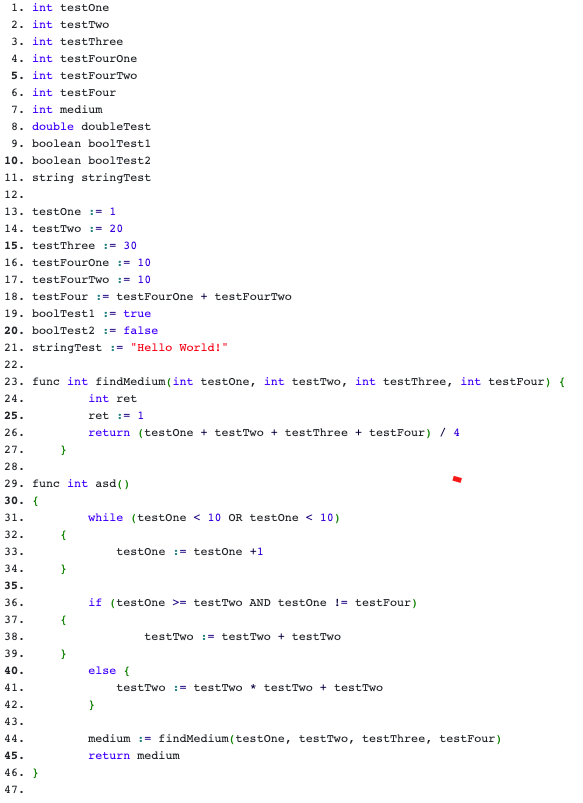
\includegraphics[scale=0.73]{figures/exp02.png}}
\caption{}
\label{ex01}
\end{figure}
The text programming example, which we will showcase in this chapter, is an example of a small recursive program, which is an example of recursion. The program itself doesn’t really have a purpose, but a good example of how recursion are used.
\begin{figure}[H]
\centering
\frame{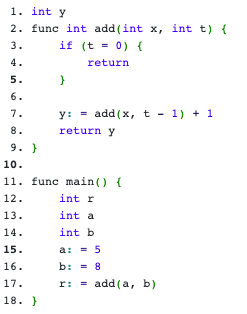
\includegraphics[scale=0.73]{figures/exp04.png}}
\caption{}
\label{ex02}
\end{figure}